\chapter{Families of Groups}
\label{chapter:families}
\thispagestyle{empty}

In this chapter we will explore a few families of groups.

\begin{section}{Cyclic Groups}

Recall that if $(G,*)$ is a group and $S\subseteq G$, then $\langle S\rangle$ the set consisting of all possible (finite) products of elements from $S$ and their inverses.  According to Theorem~\ref{thm:smallest_subgroup_containing_S}, $\langle S\rangle$ is the smallest subgroup of $G$ that contains $S$. We refer to $\langle S\rangle$ as the subgroup generated by $S$.

If we know what the elements of $S$ actually are, then we will list them inside the angle brackets without the set braces.  For example, if $S=\{a,b,c\}$, then we will write $\langle a, b, c\rangle$ instead of $\langle \{a,b,c\}\rangle$.  In this case, we refer to $\langle a, b, c\rangle$ as the subgroup generated by $a, b, c$.

In this section, we will focus on the special case when the generating set $S$ consists of a single element. If $g\in G$, then the subgroup generated by $g$ is given by
\[
\langle g\rangle =\{g^k\mid k\in\mathbb{Z}\}.
\]
We call $\langle g\rangle$ the \textbf{cyclic group generated by $g$}.  It is important to point out that $\langle g\rangle$ may be finite or infinite. In the finite case, the Cayley diagram with generator $g$ gives us a good indication of where the word ``cyclic" comes from (see Exercise~\ref{exer:Cayley_cyclic}).

\begin{exercise}
List the elements in each of the following cyclic subgroups.
\begin{enumerate}[label=\rm{(\alph*)}]
\item $\langle r\rangle$, where $r\in D_3$
\item $\langle r\rangle$, where $r\in R_4$
\item $\langle rs\rangle$, where $rs\in D_4$
\item $\langle r^2\rangle$, where $r^2\in R_6$
\item $\langle i\rangle$, where $i\in Q_8$
\item $\langle 6\rangle$, where $6\in \mathbb{Z}$ and the operation is ordinary addition
\end{enumerate}
\end{exercise}

\begin{exercise}\label{exer:subgroup_generated_by_matrix}
Consider the group of invertible $2\times 2$ matrices with real number entries under the operation of matrix multiplication.  This group is denoted $\mathrm{GL}_2(\mathbb{R})$.  List the elements in the cyclic subgroups generated by each of the following matrices.
\begin{multicols}{3}
\begin{enumerate}[label=\rm{(\alph*)}]
\item $\begin{bmatrix} 0 & -1\\ -1 & 0\end{bmatrix}$
\item $\begin{bmatrix} 0 & -1\\ 1 & 0\end{bmatrix}$
\item $\begin{bmatrix} 2 & 0\\ 0 & 1\end{bmatrix}$
\end{enumerate}
\end{multicols}
\end{exercise}

\begin{theorem}\label{thm:subgroup_generated_by_inverse}
If $(G,*)$ is a group and $g\in G$, then $\langle g\rangle=\langle g^{-1}\rangle$.
\end{theorem}

Recall that the order of a group $G$ is the number of elements in $G$. The order of $G$ is denoted $|G|$.  The next definition defines the order of an element.

\begin{definition}
Suppose $(G,*)$ is a group and let $g\in G$.  We define the \textbf{order} of $g$, written $|g|$, to be the order of $\langle g\rangle$.  That is, $|g|=|\langle g\rangle|$.
\end{definition}

\begin{exercise}
What is the order of the identity in any group?
\end{exercise}

\begin{exercise}\label{exer:computing_orders}
Find the orders of each of the elements in each of the following groups.
\begin{multicols}{2}
\begin{enumerate}[label=\rm{(\alph*)}]
\item $S_2$
\item $R_3$
\item $R_4$
\item $V_4$
\item $R_5$
\item $R_6$
\item $D_3$
\item $R_7$
\item $R_8$
\item $\Spin_{1\times 2}$
\item $D_4$
\item $Q_8$
\end{enumerate}
\end{multicols}
\end{exercise}

\begin{exercise}
Consider the group $(\mathbb{Z},+)$.  What is the order of 1?  Are there any elements in $\mathbb{Z}$ with finite order?
\end{exercise}

\begin{exercise}
Find the order of each of the matrices in Exercise~\ref{exer:subgroup_generated_by_matrix}.
\end{exercise}

The next result follows immediately from Theorem~\ref{thm:subgroup_generated_by_inverse}.

\begin{theorem}
If $(G,*)$ is a group and $g\in G$, then $|g|=|g^{-1}|$.
\end{theorem}

If $G$ is a group and $g\in G$, then there are two possibilities for $\langle g\rangle$. If all the powers $g^k$ are distinct, then it must be the case that $\langle g\rangle$ is an infinite group. The other possibility is that there exists two powers of $g$ that coincide. Suppose there exists $k<m$ such that $g^m=g^k$. Multiplying both sides of this equation by the inverse of $g^k$ yields $g^{m-k}=e$. Notice that since $k<m$, the exponent $m-k$ is positive regardless of whether $k$ and $m$ are positive or negative. We have shown that if there exists two different powers of $g$ that are equal, then there exists a positive power of $g$ that equals the identity. 

Suppose $n$ is the smallest positive integer such that $g^n=e$.  We will argue that the elements $e, g, g^2, \ldots, g^{n-1}$ are all distinct. For sake of a contradiction, assume $g^m=g^k$, where $0\leq k< m \leq n-1$. By the same reasoning as the paragraph above, it follows that $g^{m-k}=e$.  However, this contradicts the minimality of $n$ since $0<m-k<n$.

The last few paragraphs justify the following theorem.

\begin{theorem}
Suppose $(G,*)$ is a group and let $g\in G$.
\begin{enumerate}[label=\rm{(\alph*)}]
\item The subgroup $\langle g\rangle$ is infinite if and only if each $g^k$ is distinct for all $k\in\mathbb{Z}$.
\item The subgroup $\langle g\rangle$ is finite if and only if there exists a positive integer $n$ such that $g^n=e$. Moreover, if $n$ is the smallest positive integer such that $g^n=e$, then the elements $e, g, g^2, \ldots, g^{n-1}$ are all distinct.
\end{enumerate}
\end{theorem}

The next result should look familiar and will come in handy a few times in this chapter.  In particular, it will be useful when proving Theorems~\ref{thm:finite_cyclic_subgroup}, \ref{thm:criterion_on_powers}, and \ref{thm:subgroups_of_cyclic_groups}.  We'll take the result for granted and not worry about proving it.

\begin{theorem}[Division Algorithm]
If $m$ is a positive integer and $n$ is any integer, then there exist unique integers $q$ (called the \textbf{quotient}) and $r$ (called the \textbf{remainder}) such that $n=mq+r$, where $0\leq r<m$.
\end{theorem}

Use the Division Algorithm to prove the following theorem.

\begin{theorem}\label{thm:finite_cyclic_subgroup}
Suppose $(G,*)$ is a group and let $g\in G$ such that $\langle g\rangle$ is finite.  If $n$ is the smallest positive exponent such that $g^n=e$, then $\langle g\rangle = \{e, g, g^2, \ldots, g^{n-1}\}$.
\end{theorem}

The next result provides an extremely useful interpretation of the order of an element.

\begin{corollary}
If $(G,*)$ is a finite group and $g\in G$, then the order of $g$ is the smallest positive integer $n$ such that $g^n=e$.
\end{corollary}

\begin{exercise}\label{exer:Cayley_cyclic}
Suppose $\langle g\rangle$ is a finite group.  Since $\langle g\rangle$ is a group in its own right, we can draw a Cayley diagram for this group.  Using the generator $g$, what does the Cayley diagram for $\langle g\rangle$ look like?
\end{exercise}

\begin{exercise}\label{exer:finite_pos_exps}
Notice that in the definition for $\langle g\rangle$, we allow the exponents on $g$ to be negative.  Explain why we only need to use positive exponents when $\langle g\rangle$ is a finite group.
\end{exercise}

\begin{exercise}\label{exer:MultiplesOfOrder}
Suppose $(G,*)$ is a group $g\in G$ with $|g|=n$.  For what other exponents $k$ do you think will it be true that $g^k=e$? You'll have an opportunity to prove your claim later.
\end{exercise}

We are finally ready to introduce our family of interest for this section.

\begin{definition}
Suppose $(G,*)$ is a group.  Then we say that $G$ is a \textbf{cyclic group} if and only if there exists $g\in G$ such that $\langle g\rangle =G$.
\end{definition}

It is clear that if $G$ is cyclic with generator $g$, then $|G|=|g|$.  In fact, if $g\in G$, the converse is true, as well.

\begin{exercise}
Determine whether each of the groups from Exercise~\ref{exer:computing_orders} are cyclic.  If the group is cyclic, find at least one generator.
\end{exercise}

\begin{exercise}
Determine whether each of the following groups are cyclic.  If the group is cyclic, find at least one generator. If you believe that a group is not cyclic, try to sketch an argument.
\begin{multicols}{2}
\begin{enumerate}[label=\rm{(\alph*)}]
\item $(\mathbb{Z},+)$
\item $(\mathbb{R},+)$
\item $(\mathbb{R}^+,\cdot)$
\item $(\{6^n\mid n\in\mathbb{Z}\},\cdot)$
\end{enumerate}
\end{multicols}
\begin{enumerate}
\item[(e)] $\textrm{GL}_2(\mathbb{R})$ under matrix multiplication
\item[(f)] $\{(\cos(\pi/4) +i\sin(\pi/4))^n\mid n\in \mathbb{Z}\}$ under multiplication of complex numbers
\end{enumerate}
\end{exercise}

\begin{theorem}
If $(G,*)$ is a cyclic group, then $G$ is abelian.
\end{theorem}

\begin{exercise}
Provide an example of a finite group that is abelian but not cyclic.
\end{exercise}

\begin{exercise}
Provide an example of an infinite group that is abelian but not cyclic.
\end{exercise}

\begin{theorem}
If $(G,*)$ is a cyclic group such that $G$ has exactly one element that generates all of $G$, then the order of $G$ is at most order 2.   
\end{theorem}

\begin{theorem}
If $(G,*)$ is a group such that $G$ has no proper nontrivial subgroups, then $G$ is cyclic.
\end{theorem}

\begin{theorem}\label{thm:infinite_cyclic_groups}
If $(G,*)$ is an infinite cyclic group, then $G$ is isomorphic to $\mathbb{Z}$ (under the operation of addition).
\end{theorem}

Recall that for $n\geq3$, $R_n$ is the group of rotational symmetries of a regular $n$-gon, where the operation is composition of actions.

\begin{theorem}
For all $n\geq 3$, $R_n$ is cyclic.
\end{theorem}

\begin{theorem}\label{thm:finite_cyclic_groups}
Suppose $(G,*)$ is a finite cyclic group of order $n\geq 1$.  Then $G$ is isomorphic to $R_n$ if $n\geq 3$, $S_2$ if $n=2$, and the trivial group if $n=1$.
\end{theorem}

The upshot of Theorems~\ref{thm:infinite_cyclic_groups} and \ref{thm:finite_cyclic_groups} is that up to isomorphism, we know exactly what all of the cyclic groups are.

\begin{exercise}
Suppose $(G,*)$ is a finite cyclic group of order $n$ with generator $a$.  If we write down the group table for $G$ using $e, a, a^2, \ldots, a^{n-1}$ as the labels for the rows and columns, are there any interesting patterns in the table?
\end{exercise}

Recall that two integers are \textbf{relatively prime} if they have no factors other than 1 in common.  That is, integers $n$ and $k$ are relatively prime if and only if $\gcd(n,k)=1$.

\begin{definition}
Let $n\in\mathbb{N}$ and define the following sets.
\begin{enumerate}[label=\rm{(\alph*)}]
\item $\mathbb{Z}_n:=\{0,1,\ldots,n-1\}$
\item $U(n):=\{k\in\mathbb{Z}_n\mid \gcd(n,k)=1\}$
\end{enumerate}
\end{definition}

For each set above, the immediate goal is to find a binary operation that will yield a group.  The key is to use modular arithmetic.  To calculate the sum (respectively, product) of two integers mod $n$, add (respectively, multiply) the two numbers and then find the remainder after dividing the sum (respectively, product) by $n$. For example, $4+9$ is $3$ mod $5$ since $13$ has remainder 3 when being divided by 5.  Similarly, $4\cdot 9$ is 1 mod $5$ since 36 has remainder 1 when being divided by 5.

\begin{theorem}
The set $\mathbb{Z}_n$ is a group under addition mod $n$.  
\end{theorem}

\begin{theorem}
The set $U(n)$ is a group under multiplication mod $n$.  
\end{theorem}

\begin{exercise}
Consider $\mathbb{Z}_4$.
\begin{enumerate}[label=\rm{(\alph*)}]
\item Find the group table for $\mathbb{Z}_4$.
\item Is $\mathbb{Z}_4$ cyclic? If so, list elements of $\mathbb{Z}_4$ that individually generate $\mathbb{Z}_4$.  If $\mathbb{Z}_4$ is not cyclic, explain why.
\item Is $\mathbb{Z}_4$ isomorphic to either of $R_4$ or $V_4$? Justify your answer.
\item Draw the subgroup lattice for $\mathbb{Z}_4$.
\end{enumerate}
\end{exercise}

\begin{exercise}\label{exer:U10}
Consider $U(10)=\{1,3,7,9\}$.
\begin{enumerate}[label=\rm{(\alph*)}]
\item Find the group table for $U(10)$.
\item Is $U(10)$ cyclic? If so, list elements of $U(10)$ that individually generate $U(10)$.  If $U(10)$ is not cyclic, explain why.
\item Is $U(10)$ isomorphic to either of $R_4$ or $V_4$? Justify your answer.
\item Is $U(10)$ isomorphic to $\mathbb{Z}_4$? Justify your answer.
\item Draw the subgroup lattice for $U(10)$.
\end{enumerate}
\end{exercise}

\begin{exercise}\label{exer:U12}
Consider $U(12)=\{1,5,7,11\}$.
\begin{enumerate}[label=\rm{(\alph*)}]
\item Find the group table for $U(12)$.
\item Is $U(12)$ cyclic? If so, list elements of $U(12)$ that individually generate $U(12)$.  If $U(12)$ is not cyclic, explain why.
\item Is $U(12)$ isomorphic to either of $R_4$ or $V_4$? Justify your answer.
\item Draw the subgroup lattice for $U(12)$.
\end{enumerate}
\end{exercise}

In light of Exercises~\ref{exer:U10} and \ref{exer:U12}, $U(n)$ may or may not be cyclic. Nonetheless, as the next theorem illustrates, $U(n)$ is always abelian.

\begin{theorem}
For all $n$, $U(n)$ is abelian.
\end{theorem}

The upshot of the next theorem is that for $n\geq 3$, $\mathbb{Z}_n$ is just the set of (smallest nonnegative) exponents on $r$ in $R_n$.

\begin{theorem}\label{thm:Zn_iso_to_Rn}
For $n\geq 3$, $\mathbb{Z}_n\cong R_n$. Moreover, $\mathbb{Z}_2\cong S_2$ and $\mathbb{Z}_1$ is isomorphic to the trivial group.
\end{theorem}

One consequence of the previous theorem is that $\mathbb{Z}_n$ is always cyclic. Combining the results of Theorems~\ref{thm:finite_cyclic_groups} and \ref{thm:infinite_cyclic_groups} together with Theorem~\ref{thm:Zn_iso_to_Rn}, we immediately obtain the following.

\begin{theorem}
Let $(G,*)$ be a cyclic group. If the order of $G$ is infinite, then $(G,*)$ is isomorphic to $(\mathbb{Z},+)$. If $G$ has finite order $n$, then $(G,*)$ is isomorphic to $(\mathbb{Z}_n,+\text{ mod }n)$.
\end{theorem}

Now that we have a complete description of the cyclic groups, let's focus our attention on subgroups of cyclic groups.  The Division Algorithm should come in handy when proving the next theorem.

\begin{theorem}\label{thm:criterion_on_powers}
Suppose $(G,*)$ is a group and let $a\in G$ such that $|a|=n$.  Then $a^i=a^j$ if and only if $n$ divides $i-j$.
\end{theorem}

Compare the next result to Exercise~\ref{exer:MultiplesOfOrder}.

\begin{corollary}
Suppose $(G,*)$ is a group and let $a\in G$ such that $|a|=n$.  If $a^k=e$, then $|a|$ divides $k$.
\end{corollary}

\begin{theorem}\label{thm:subgroups_of_cyclic_groups}
Suppose $(G,*)$ is a cyclic group. If $H\leq G$, then $H$ is also cyclic.
\end{theorem}

It turns out that for proper subgroups, the converse of Theorem~\ref{thm:subgroups_of_cyclic_groups} is not true.

\begin{exercise}
Provide an example of a group $(G,*)$ such that $G$ is not cyclic, but all proper subgroups of $G$ are cyclic.
\end{exercise}

The next result officially settles Exercise~\ref{exer:nZ}\ref{exer:nZothers} and also provides a complete description of the subgroups of infinite cyclic groups up to isomorphism.

\begin{corollary}\label{cor:subgroups_of_Z}
The subgroups of $\mathbb{Z}$ are precisely the groups $n\mathbb{Z}$ under addition for $n\in \mathbb{Z}$.
\end{corollary}

What about finite cyclic groups?

\begin{theorem}
Suppose $(G,*)$ is a finite cyclic group with generator $a$ such that $|G|=n$.  
\begin{enumerate}[label=\rm{(\alph*)}]
\item Then $\displaystyle |a^s|=\frac{n}{\gcd(n,s)}$.
\item Moreover, $\langle a^s\rangle=\langle a^t\rangle$ if and only if $\gcd(s,n)=\gcd(t,n)$.
\end{enumerate}
\end{theorem}

\begin{exercise}
Suppose $(G,*)$ is a cyclic group of order 12 with generator $a$. 
\begin{enumerate}[label=\rm{(\alph*)}]
\item Find the orders of each of the following elements: $a^2$, $a^7$, $a^8$.
\item Which elements of $G$ individually generate $G$?
\end{enumerate}
\end{exercise}

\begin{corollary}
Suppose $(G,*)$ is a finite cyclic group with generator $a$ such that $|G|=n$. Then $\langle a\rangle=\langle a^r\rangle$ if and only if $n$ and $r$ are relatively prime. That is, $a^r$ generates $G$ if and only if $n$ and $r$ are relatively prime.
\end{corollary}

\begin{exercise}
Consider $(\mathbb{Z}_{18},+\text{ mod }18)$.
\begin{enumerate}[label=\rm{(\alph*)}]
\item Find all of the elements of $\mathbb{Z}_{18}$ that individually generate all of $\mathbb{Z}_{18}$.
\item Draw the subgroup lattice for $\mathbb{Z}_{18}$. For each subgroup, list the elements of the corresponding set.  Moreover, circle the the elements in each subgroup that individually generate that subgroup.  For example, $\langle 2\rangle=\{0,2,4,6,8,10,12,14,16\}$. In this case, we should circle 2, 4, 8, 10, 14, and 16 since each of these elements individually generate $\langle 2\rangle$ and none of the remaining elements do.  I'll leave it to you to figure out why this is true.
\end{enumerate}
\end{exercise}

\begin{exercise}
Repeat the above exercise, but this time use $\mathbb{Z}_{12}$ instead of $\mathbb{Z}_{18}$.
\end{exercise}

\begin{corollary}
Suppose $(G,*)$ is a finite cyclic group such that $|G|=p$, where $p$ is prime. Then $G$ has no proper nontrivial subgroups.
\end{corollary}

\begin{problem}
Let $p$ and $q$ be distinct primes. Find the number of generators of $\mathbb{Z}_{pq}$.
\end{problem}

\begin{problem}
Let $p$ be a prime. Find the number of generators of $\mathbb{Z}_{p^r}$, where $r$ is an integer greater than or equal to 1.
\end{problem}

\begin{problem}
If there is exactly one group up to isomorphism of order $n$, then to what group are all the groups of order $n$ isomorphic?
\end{problem}

\end{section}

\begin{section}{Dihedral Groups}

We can think of finite cyclic groups as groups that describe rotational symmetry.  In particular, $R_n$ is the group of rotational symmetries of a regular $n$-gon.  Dihedral groups are those groups that describe both rotational and reflectional symmetry of regular $n$-gons.

\begin{definition}\label{def:dihedral}
For $n\geq 3$, the \textbf{dihedral group} $D_n$ is defined to be the group consisting of the symmetry actions of a regular $n$-gon, where the operation is composition of actions.
\end{definition}

For example, as we've seen, $D_3$ and $D_4$ are the symmetry groups of equilateral triangles and squares, respectively.  The symmetry group of a regular pentagon is denoted by $D_5$.  It is a well-known fact from geometry that the composition of two reflections in the plane is a rotation by twice the angle between the reflecting lines.

\begin{theorem}
The group $D_n$ is a non-abelian group of order $2n$.
\end{theorem}

\begin{theorem}
For $n\geq 3$, $R_n\leq D_n$.
\end{theorem}

\begin{theorem}\label{thm:generators_Dn}
Fix $n\geq 3$ and consider $D_n$. Let $r$ be rotation clockwise by $360^{\circ}/n$  and let $s$ and $s'$ be any two adjacent reflections of a regular $n$-gon.  Then
\begin{enumerate}[label=\rm{(\alph*)}]
\item $D_n=\langle r,s\rangle =\{\underbrace{e,r,r^2,\ldots, r^{n-1}}_{\text{rotations}},\underbrace{s,sr,sr^2,\ldots,sr^{n-1}}_{\text{reflections}}\}$ and
\item $D_n=\langle s,s'\rangle = \text{all possible products of }s\text{ and }s'$.
\end{enumerate}
\end{theorem}

\begin{theorem}
Fix $n\geq 3$ and consider $D_n$. Let $r$ be rotation clockwise by $360^{\circ}/n$  and let $s$ and $s'$ be any two adjacent reflections of a regular $n$-gon.  Then the following relations hold.
\begin{enumerate}[label=\rm{(\alph*)}]
\item $r^n = s^2 = (s')^2 =e$,
\item $r^{-k} = r^{n-k}$ (special case: $r^{-1}=r^{n-1}$),
\item $sr^k=r^{n-k}s$ (special case: $sr=r^{n-1}s$),
\item $\underbrace{ss's\cdots}_{n\text{ factors}}=\underbrace{s'ss'\cdots}_{n\text{ factors}}$.
\end{enumerate}
\end{theorem}

\begin{exercise}
From Theorem~\ref{thm:generators_Dn}, we know
\[
D_n=\langle r,s\rangle =\{\underbrace{e,r,r^2,\ldots, r^{n-1}}_{\text{rotations}},\underbrace{s,sr,sr^2,\ldots,sr^{n-1}}_{\text{reflections}}\}.
\]
If you were to create the group table for $D_n$ so that the rows and columns of the table were labeled by $e,r,r^2,\ldots, r^{n-1},s,sr,sr^2,\ldots,sr^{n-1}$ (in exactly that order), do any patterns arise?  \emph{Hint:} Where are the rotations? Where are the reflections?
\end{exercise}

\begin{exercise}
What does the Cayley diagram for $D_n$ look like if we use $\{r,s\}$ as the generating set?  What if we use $\{s,s'\}$ as the generating set?
\end{exercise}

\end{section}

\begin{section}{Symmetric Groups}

Recall the group $S_3$ from Exercise~\ref{exer:S3}.  This group acts on three coins that are in a row by rearranging their positions (but not flipping them over). This group is an example of a \textbf{symmetric group}.  In general, the symmetric group on $n$ objects is the set of permutations that rearranges the $n$ objects.  The group operation is composition of permutations.  Let's be a little more formal.

\begin{definition}
A \textbf{permutation of a set $A$} is a function $\sigma:A\to A$ that is both one-to-one and onto.
\end{definition}

You should take a moment to convince yourself that the formal definition of a permutation agrees with the notion of rearranging the set of objects.  The do-nothing action is the identity permutation, i.e., $\sigma(a)=a$ for all $a\in A$.  There are many ways to represent a permutation.  One visual way is using \textbf{permutation diagrams}, which we will introduce via examples.

Consider the following diagrams:
\begin{multicols}{2}
\[\alpha=\begin{pdiag}{5}{1}
\put(0.2,2.3){{1}}\put(1.2,2.3){{2}}\put(2.2,2.3){{3}}\put(3.2,2.3){{4}}\put(4.2,2.3){{5}} 
\pdmap{1}{2}\pdmap{2}{3}\pdmap{3}{4}\pdmap{4}{5}\pdmap{5}{1}\pdendmapfill 
\end{pdiag}\]

\bigskip

\[\beta=\begin{pdiag}{5}{1}
\put(0.2,2.3){{1}}\put(1.2,2.3){{2}}\put(2.2,2.3){{3}}\put(3.2,2.3){{4}}\put(4.2,2.3){{5}} 
\pdmap{2}{4}\pdmap{4}{3}\pdmap{3}{2}\pdendmapfill 
\end{pdiag}\]

\[\sigma=\begin{pdiag}{5}{1}
\put(0.2,2.3){{1}}\put(1.2,2.3){{2}}\put(2.2,2.3){{3}}\put(3.2,2.3){{4}}\put(4.2,2.3){{5}} 
\pdtrans{1}{3}\pdmap{2}{5}\pdmap{5}{4}\pdmap{4}{2}\pdendmapfill 
\end{pdiag}\]

\bigskip

\[\gamma=\begin{pdiag}{5}{1}
\put(0.2,2.3){{1}}\put(1.2,2.3){{2}}\put(2.2,2.3){{3}}\put(3.2,2.3){{4}}\put(4.2,2.3){{5}}
\pdtrans{1}{5}\pdendmapfill 
\end{pdiag}\]
\end{multicols}
\noindent Each of these diagrams represents a permutation on five objects.  I've given the permutations the names $\alpha$, $\beta$, $\sigma$, and $\gamma$.  The intention is to read the diagrams from the top down.  The numbers labeling the nodes along the top are identifying position.  Following an edge from the top row of nodes to the bottom row of nodes tells us what position an object moves to.  It is important to remember that the numbers are referring to the position of an object, not the object itself.  For example, $\beta$ is the permutation that sends the object in the second position to the fourth position, the object in the third position to the second position, and the object in the fourth position to the third position.  Moreover, the permutation $\beta$ doesn't do anything to the objects in positions 1 and 5.

\begin{exercise}
Describe in words what the permutations $\sigma$ and $\gamma$ do.
\end{exercise}

\begin{exercise}
Draw the permutation diagram for the do-nothing permutation on 5 objects.  This is called the \textbf{identity permutation}. What does the identity permutation diagram look like in general for arbitrary $n$?
\end{exercise}

\begin{definition}
The set of all permutations on $n$ objects is denoted by $S_n$.
\end{definition}

\begin{exercise}
Draw all the permutation diagrams for the permutations in $S_3$.
\end{exercise}

\begin{exercise}
How many distinct permutations are there in $S_4$?  How about $S_n$ for any $n\in \mathbb{N}$?
\end{exercise}

If $S_n$ is going to be a group, we need to know how to compose permutations.  This is easy to do using the permutation diagrams.  Consider the permutations $\alpha$ and $\beta$ from earlier.  We can represent the composition $\alpha \circ \beta$ via

\bigskip

\[\alpha \circ \beta=\begin{pdiag}{5}{2}
\put(0.2,4.3){{1}}\put(1.2,4.3){{2}}\put(2.2,4.3){{3}}\put(3.2,4.3){{4}}\put(4.2,4.3){{5}} 
\pdname{\tiny \beta}\pdmap{2}{4}\pdmap{4}{3}\pdmap{3}{2}\pdendmapfill 
\pdname{\tiny \alpha}\pdmap{1}{2}\pdmap{2}{3}\pdmap{3}{4}\pdmap{4}{5}\pdmap{5}{1}\pdendmapfill 
\end{pdiag}=
\begin{pdiag}{5}{1}
\put(0.2,2.3){{1}}\put(1.2,2.3){{2}}\put(2.2,2.3){{3}}\put(3.2,2.3){{4}}\put(4.2,2.3){{5}} 
\pdmap{1}{2}\pdmap{2}{5}\pdmap{5}{1}\pdendmapfill 
\end{pdiag}.\]
\noindent As you can see by looking at the figure, to compose two permutations, you stack the one that goes first in the composition (e.g., $\beta$ in the example above) on top of the other and just follow the edges from the top through the middle to the bottom.  If you think about how function composition works, this is very natural.  The resulting permutation is determined by where we begin and where we end in the composition.

We already know that the order of composition matters for functions, and so it should matter for the composition of permutations. To make this crystal clear, let's compose $\alpha$ and $\beta$ in the opposite order.  We see that

\bigskip

\[\beta \circ \alpha=\begin{pdiag}{5}{2}
\put(0.2,4.3){{1}}\put(1.2,4.3){{2}}\put(2.2,4.3){{3}}\put(3.2,4.3){{4}}\put(4.2,4.3){{5}} 
\pdname{\tiny \alpha}\pdmap{1}{2}\pdmap{2}{3}\pdmap{3}{4}\pdmap{4}{5}\pdmap{5}{1}\pdendmapfill 
\pdname{\tiny \beta}\pdmap{2}{4}\pdmap{4}{3}\pdmap{3}{2}\pdendmapfill 
\end{pdiag}=
\begin{pdiag}{5}{1}
\put(0.2,2.3){{1}}\put(1.2,2.3){{2}}\put(2.2,2.3){{3}}\put(3.2,2.3){{4}}\put(4.2,2.3){{5}} 
\pdmap{1}{4}\pdmap{4}{5}\pdmap{5}{1}\pdendmapfill 
\end{pdiag}.\]

\noindent The moral of the story is that composition of permutations does not necessarily commute.

\begin{exercise}
Consider $\alpha$, $\beta$, $\sigma$, and $\gamma$ from earlier.  Can you find a pair of permutations that do commute?  Can you identify any features about your diagrams that indicate why they commuted?
\end{exercise}

\begin{exercise}
Fix $n\in\mathbb{N}$.  Convince yourself that any $\rho\in S_n$ composed with the identity permutation (in either order) equals $\rho$.
\end{exercise}

If $S_n$ is going to be a group, we need to know what the inverse of a permutation is.

\begin{problem}
Given a permutation $\rho\in S_n$, describe a method for constructing $\rho^{-1}$.  Briefly justify that $\rho \circ \rho^{-1}$ will yield the identity permutation.
\end{problem}

At this point, we have all the ingredients we need to prove that $S_n$ forms a group under composition of permutations.

\begin{theorem}
The set of permutations on $n$ objects forms a group under the operation of composition.  That is, $(S_n,\circ)$ is a group.  Moreover, $|S_n|=n!$.
\end{theorem}

Note that it is standard convention to omit the composition symbol when writing down compositions in $S_n$.  For example, we will simply write $\alpha\beta$ to denote $\alpha \circ \beta$.

Permutation diagrams are fun to play with, but we need a more efficient way of encoding information.  One way to do this is using \textbf{cycle notation}.  Consider $\alpha, \beta, \sigma$, and $\gamma$ in $S_{5}$ from the previous examples.  Below I have indicated what each permutation is equal to using cycle notation.

\begin{align*}\alpha=&\begin{pdiag}{5}{1} 
\pdmap{1}{2}\pdmap{2}{3}\pdmap{3}{4}\pdmap{4}{5}\pdmap{5}{1}\pdendmapfill 
\end{pdiag}=\ (1,2,3,4,5)\\
\\
\beta=&\begin{pdiag}{5}{1} 
\pdmap{2}{4}\pdmap{4}{3}\pdmap{3}{2}\pdendmapfill 
\end{pdiag}=\ (2,4,3)\\
\\
\sigma=&\begin{pdiag}{5}{1} 
\pdtrans{1}{3}\pdmap{2}{5}\pdmap{5}{4}\pdmap{4}{2}\pdendmapfill 
\end{pdiag}=\ (1,3)(2,5,4)\\
\\
\gamma=&\begin{pdiag}{5}{1} 
\pdtrans{1}{5}\pdendmapfill 
\end{pdiag}=\ (1,5)
\end{align*}
Each string of numbers enclosed by parentheses is called a \textbf{cycle} and if the string of numbers has length $k$, then we call it a $k$-cycle.  For example, $\alpha$ consists of a single 5-cycle, whereas $\sigma$ consists of one 2-cycle and one 3-cycle.  In the case of $\sigma$, we say that $\sigma$ is the product of two \textbf{disjoint cycles}.  

One observation that you hopefully made is that if an object in position $i$ remains unchanged, then we don't bother listing that number in the cycle notation.  However, if we wanted to, we could use the 1-cycle $(i)$ to denote this.  For example, we could write $\beta=(1)(2,3,4)(5)$.  In particular, we could denote the identity permutation in $S_5$ using $(1)(2)(3)(4)(5)$.  Yet, it is common to simply use $(1)$ to denote the identity in $S_n$ for all $n$.

Notice that the first number we choose to write down for a given cycle is arbitrary.  However, the numbers that follow are not negotiable.  Typically, we would use the smallest possible number first, but this is not necessary.  For example, the cycle $(2,4,7)$ could also be written as $(4,7,2)$ or $(7,2,4)$.

\begin{exercise}\label{exer:S3-2}
Write down all 6 elements in $S_3$ using cycle notation.
\end{exercise}

\begin{exercise}\label{exer:S4}
Write down all 24 elements in $S_4$ using cycle notation.
\end{exercise}

Suppose $\sigma\in S_n$.  Since $\sigma$ is one-to-one and onto, it is clear that it is possible to write $\sigma$ as a product of disjoint cycles such that each $i\in\{1,2,\ldots, n\}$ appears exactly once.

Let's see if we can figure out how to multiply elements of $S_n$ using cycle notation.  Consider the permutations $\alpha=(1,3,2)$ and $\beta=(3,4)$ in $S_4$.  To compute the composition $\alpha\beta=(1,3,2)(3,4)$, let's explore what happens in each position.  Since we are doing function composition, we should work our way from right to left.  Since 1 does not appear in the cycle notation for $\beta$, we know that $\beta(1)=1$ (i.e., $\beta$ maps 1 to 1).  Now, we see what $\alpha(1)=3$.  Thus, the composition $\alpha\beta$ maps 1 to 3 (since $\alpha\beta(1)=\alpha(\beta(1))=\alpha(1)=3$).  Next, we should return to $\beta$ and see what happens to 3---which is where we ended a moment ago.  We see that $\beta$ maps 3 to 4 and then $\alpha$ maps 4 to 4 (since 4 does not appear in the cycle notation for $\alpha$).  So, $\alpha\beta(3)=4$.  Continuing this way, we see that $\beta$ maps 4 to 3 and $\alpha$ maps 3 to 2, and so $\alpha\beta$ maps 4 to 2.  Lastly, since $\beta(2)=2$ and $\alpha(2)=1$, we have $\alpha\beta(2)=1$.  Putting this altogether, we see that $\alpha\beta=(1,3,4,2)$.  Now, you should try a few.  Things get a little trickier if the composition of two permutations results in a permutation consisting of more than a single cycle.

\begin{exercise}
Consider $\alpha$, $\beta$, $\sigma$, and $\gamma$ for which we drew the permutation diagrams.  Using cycle notation, compute each of the following.
\begin{multicols}{2}
\begin{enumerate}[label=\rm{(\alph*)}]
\item $\alpha\gamma$
\item $\alpha^2$
\item $\alpha^3$
\item $\alpha^4$
\item $\alpha^5$
\item $\sigma\alpha$
\item $\alpha^{-1}\sigma^{-1}$
\item $\beta^2$
\item $\beta^3$
\item $\beta\gamma\alpha$
\item $\sigma^3$
\item $\sigma^6$
\end{enumerate}
\end{multicols}
\end{exercise}

\begin{exercise}
Write down the group table for $S_3$ using cycle notation.
\end{exercise}

In Exercise~\ref{exer:S4}, one of the permutations you should have written down is $(1,2)(3,4)$.  This is a product of two disjoint 2-cycles.  It is worth pointing out that each cycle is a permutation in its own right.  That is, $(1,2)$ and $(3,4)$ are each permutations.  It just so happens that their composition does not ``simplify" any further.  Moreover, these two disjoint 2-cycles commute since $(1,2)(3,4)=(3,4)(1,2)$.  In fact, this phenomenon is always true.

\begin{theorem}
Suppose $\alpha$ and $\beta$ are two disjoint cycles.  Then $\alpha\beta=\beta\alpha$.  That is, products of disjoint cycles commute.
\end{theorem}

Computing the order of a permutation is fairly easy using cycle notation once we figure out how to do it for a single cycle.  In fact, you've probably already guessed at the following theorem.

\begin{theorem}
Suppose $\alpha\in S_n$ such that $\alpha$ consists of a single $k$-cycle.  Then $|\alpha|=k$.
\end{theorem}

\begin{theorem}
Suppose $\alpha\in S_n$ such that $\alpha$ consists of $m$ disjoint cycles of lengths $k_1,\ldots, k_m$.  Then $|\alpha|=\lcm(k_1,\ldots, k_m)$.\footnote{Recall that $\lcm(k_1,\ldots, k_m)$ is the \textbf{least common multiple} of $\{k_1,\ldots, k_m\}$.} 
\end{theorem}

\begin{problem}
Is the previous theorem true if we do not require the cycles to be disjoint?  Justify your answer.
\end{problem}

\begin{exercise}
Compute the orders of all the elements in $S_3$.  See Exercise~\ref{exer:S3-2}.
\end{exercise}

\begin{exercise}
Compute the orders of all the elements in $S_4$.  See Exercise~\ref{exer:S4}.
\end{exercise}

\begin{exercise}
What is the order of $(1,4,7)(2,5)(3,6,8,9)$?
\end{exercise}

\begin{exercise}
Draw the subgroup lattice for $S_3$.
\end{exercise}

\begin{exercise}
Now, using $(1,2)$ and $(1,2,3)$ as generators, draw the Cayley diagram for $S_3$.  Look familiar?
\end{exercise}

It turns out that the subgroups of symmetric groups play an important role in group theory.

\begin{definition}
Every subgroup of a symmetric group is called a \textbf{permutation group}.
\end{definition}

The proof of the following theorem isn't too bad, but for now we'll take it for granted.

\begin{theorem}[Cayley's Theorem]
Every finite group is isomorphic to some permutation group.  In particular, if $(G,*)$ is a group of order $n$, then $G$ is isomorphic to a subgroup of $S_n$.
\end{theorem}

Cayley's Theorem guarantees that every finite group is isomorphic to a permutation group and it turns out that there is a rather simple algorithm for constructing the corresponding permutation group.  I'll briefly explain an example and then let you try a couple.

Consider the Klein four-group $V_4=\{e,v,h,vh\}$.  Recall that $V_4$ has the following group table.

\begin{center}
\begin{tabu}{c|[2pt]c|c|c|c}
$*$ & $e$ & $v$ & $h$ & $vh$ \\ \tabucline[2pt]{-}
$e$ & $e$ & $v$ & $h$ & $vh$ \\
\hline $v$ & $v$ & $e$ & $vh$ & $h$  \\
\hline $h$ & $h$ & $vh$ & $e$ & $v$\\
\hline $vh$ & $vh$ & $h$ & $v$ & $e$
\end{tabu}
\end{center}

If we number the elements $e,v,h,$ and $vh$ as $1,2,3,$ and $4$, respectively, then we obtain the following table.

\begin{center}
\begin{tabu}{c|[2pt]c|c|c|c}
 & $1$ & $2$ & $3$ & $4$ \\ \tabucline[2pt]{-}
$1$ & $1$ & $2$ & $3$ & $4$ \\
\hline $2$ & $2$ & $1$ & $4$ & $3$  \\
\hline $3$ & $3$ & $4$ & $1$ & $2$\\
\hline $4$ & $4$ & $3$ & $2$ & $1$
\end{tabu}
\end{center}

\noindent Comparing each of the four columns to the leftmost column, we can obtain the corresponding permutations.  In particular, we obtain
\begin{align*}
e&\leftrightarrow (1)\\
v&\leftrightarrow (1,2)(3,4)\\
h&\leftrightarrow (1,3)(2,4)\\
vh&\leftrightarrow(1,4)(2,3). 
\end{align*}
Do you see where these permutations came from?  The claim is that the set of permutations $\{(1),(1,2)(3,4),(1,3)(2,4),(1,4)(2,3)\}$ is isomorphic to $V_4$.  In this particular case, it's fairly clear that this is true.  However, it takes some work to prove that this process will always result in an isomorphic permutation group.  In fact, verifying the algorithm is essentially the proof of Cayley's Theorem. 

Since there are potentially many ways to rearrange the rows and columns of a given table, it should be clear that there are potentially many isomorphisms that could result from the algorithm described above.

Here's another way to obtain a permutation group that is isomorphic to a given group.  Let's consider $V_4$ again.  Recall that $V_4$ is a subset of $D_4$, which is the symmetry group for a square.  Alternatively, $V_4$ is the symmetry group for a non-square rectangle.  Label the corners of the rectangle 1, 2, 3, and 4 by starting in the upper left corner and continuing clockwise.  Recall that $v$ is the action that reflects the rectangle over the vertical midline.  The result of this action is that the corners labeled by 1 and 2 switch places and the corners labeled by 3 and 4 switch places.  Thus, $v$ corresponds to the permutation $(1,2)(3,4)$.  Similarly, $h$ swaps the corners labeled by 1 and 4 and the corners labeled by 2 and 3, and so $h$ corresponds to the permutation $(1,4)(2,3)$.  Notice that this is not the same answer we got earlier and that's okay as there may be many permutation representations for a given group.  Lastly, $vh$ rotates the rectangle $180^{\circ}$ which sends ends up swapping corners labeled 1 and 3 and swapping corners labeled by 2 and 4.  Therefore, $vh$ corresponds to the permutation $(1,3)(2,4)$.

\begin{exercise}
Find a permutation group that is isomorphic to $D_4$.
\end{exercise}

\begin{exercise}
Find a permutation group that is isomorphic to $\mathbb{Z}_6$.
\end{exercise}

\begin{exercise}
Consider $S_3$.
\begin{enumerate}[label=\rm{(\alph*)}]
\item Using $(1,2)$, $(1,3)$, and $(2,3)$ as generators, draw the Cayley diagram for $S_3$.
\item In the previous part, we used a generating set with three elements.  Is there a smaller generating set?  If so, what is it?
\end{enumerate}
\end{exercise}

\begin{exercise}
Recall that there are $4!=24$ permutations in $S_4$.    
\begin{enumerate}[label=\rm{(\alph*)}]
\item Pick any 12 permutations from $S_4$ and verify that you can write them as words in the 2-cycles $(1,2), (1,3), (1,4), (2,3), (2,4),(3,4)$.  In most circumstances, your words will not consist of products of disjoint 2-cycles.  For example, the permutation $(1,2,3)$ can be decomposed into $(1,2)(2,3)$, which is a word consisting of two 2-cycles that happen to not be disjoint.
\item Using your same 12 permutations, verify that you can write them as words only in the 2-cycles $(1,2),(2,3),(3,4)$.
\end{enumerate}
By the way, it might take some trial and error to come up with a way to do this.  Moreover, there is more than one way to do it.
\end{exercise}

As the previous exercises hinted at, the 2-cycles play a special role in the symmetric groups.  In fact, they have a special name.  A \textbf{transposition} is a single cycle of length 2.  In the special case that the transposition is of the form $(i,i+1)$, we call it an \textbf{adjacent transposition}.  For example, $(3,7)$ is a (non-adjacent) transposition while $(6,7)$ is an adjacent transposition.

It turns out that the set of transpositions in $S_n$ is a generating set for $S_n$.  In fact, the adjacent transpositions form an even smaller generating set for $S_n$.  To get some intuition, let's play with a few examples.

\begin{exercise}
Try to write each of the following permutations as a product of transpositions.  You do not necessarily need to use adjacent transpositions.
\begin{enumerate}[label=\rm{(\alph*)}]
\item $(3,1,5)$
\item $(2,4,6,8)$
\item $(3,1,5)(2,4,6,8)$
\item $(1,6)(2,5,3)$
\end{enumerate}
\end{exercise}

The products you found in the previous exercise are called \textbf{transposition representations} of the given permutation.

\begin{problem}
Consider the arbitrary $k$-cycle $(a_1,a_2,\ldots, a_k)$ from $S_n$ (with $k\leq n$).  Find a way to write this permutation as a product of 2-cycles. 
\end{problem}

\begin{problem}
Consider the arbitrary 2-cycle $(a,b)$ from $S_n$.  Find a way to write this permutation as a product of adjacent 2-cycles.
\end{problem}

The previous two problems imply the following theorem.

\begin{theorem}
Consider $S_n$.
\begin{enumerate}[label=\rm{(\alph*)}]
\item Every permutation in $S_n$ can be written as a product of transpositions.
\item Every permutation in $S_n$ can be written as a product of adjacent transpositions.
\end{enumerate}
\end{theorem}

\begin{corollary}
The set of transpositions (respectively, the set of adjacent transpositions) from $S_n$ forms a generating set for $S_n$.
\end{corollary}

It is important to point out that the transposition representation of a permutation is not unique.  That is, there are many words in the transpositions that will equal the same permutation.  However, as we shall see in the next section, given two transposition representations for the same permutation, the number of transpositions will have the same parity (i.e., even versus odd).

\begin{remark}
Here are two interesting facts that I will let you ponder on your own time.
\begin{enumerate}[label=\rm{(\alph*)}]
\item The group of rigid motion symmetries for a cube is isomorphic to $S_4$.  To convince yourself of this fact, first prove that this group has 24 actions and then ponder the action of $S_4$ on the four long diagonals of a cube.
\item It turns out that you can generate $S_4$ with $(1,2)$ and $(1,2,3,4)$.  Moreover, you can arrange the Cayley diagram for $S_4$ with these generators on a truncated cube, which is depicted in Figure~\ref{fig:TruncatedCube}.  Try it. 
\end{enumerate}
\end{remark}

\begin{figure}[ht!]
\begin{center}
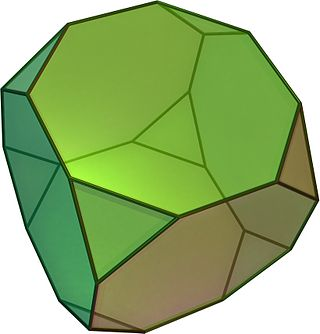
\includegraphics[width=2in]{TruncatedCube.jpg}
\end{center}
\caption{Truncated cube. [Image source: \href{https://en.wikipedia.org/wiki/Truncated_cube}{Wikipedia}]}\label{fig:TruncatedCube}
\end{figure}

\end{section}

\begin{section}{Alternating Groups}

In this section, we describe a special class of permutation groups.  To get started, let's play with a few exercises.

\begin{exercise}
Write down every permutation in $S_3$ as a product of 2-cycles in the most efficient way you can find (i.e., use the fewest possible transpositions).  Now, write every permutation in $S_3$ as a product of adjacent 2-cycles, but don't worry about whether your decompositions are efficient.  Any observations about the number of transpositions you used in each case?  Think about even versus odd.
\end{exercise}

\begin{lemma}
Suppose $\alpha_1,\alpha_2,\ldots,\alpha_k$ is a collection of 2-cycles in $S_n$ such that $\alpha_1\alpha_2\cdots\alpha_k=(1)$.  Then $k$ must be even.  \emph{Hint:} Use strong induction on $k$. Start by showing that $k\neq 1$ but that the statement is true when $k=2$. Then assume that $k>2$ and proceed by induction.
\end{lemma}

\begin{theorem}
If $\sigma\in S_n$, then every transposition representation of $\sigma$ has the same parity.
\end{theorem}

The previous theorem tells us that the following definition is well-defined.

\begin{definition}
A permutation is \textbf{even} (respectively, \textbf{odd}) if one of its transposition representations consists of an even (respectively, odd) number of transpositions.
\end{definition}

\begin{exercise}
Classify all of the permutations in $S_3$ as even or odd.
\end{exercise}

\begin{exercise}
Classify all of the permutations in $S_4$ as even or odd.
\end{exercise}

\begin{exercise}
Determine whether $(1,4,2,3,5)$ is even or odd.  How about $(1,4,2,3,5)(7,9)$?
\end{exercise}

\begin{problem}
Consider the arbitrary $k$-cycle $(a_1,a_2,\ldots, a_k)$ from $S_n$ (with $k\leq n$).  When will this cycle be odd versus even?  Briefly justify your answer. 
\end{problem}

\begin{problem}
Conjecture a statement about when a permutation will be even versus odd.  Briefly justify your answer.
\end{problem}

And finally, we are ready to introduce the alternating groups.

\begin{definition}
The set of all even permutations in $S_n$ is denoted by $A_n$ and is called the \textbf{alternating group}.
\end{definition}

Since we referred to $A_n$ as a group, it darn well better be a group!

\begin{theorem}
The set $A_n$ forms a group under composition of permutations and has order $n!/2$.
\end{theorem}

\begin{exercise}
Find $A_3$.  What group is $A_3$ isomorphic to?
\end{exercise}

\begin{exercise}
Find $A_4$ and then draw its subgroup lattice. Is $A_4$ abelian?
\end{exercise}

\begin{exercise}
What is the order of $A_5$?  Is $A_5$ abelian?
\end{exercise}

\begin{exercise}
What are the possible orders for elements in $S_6$ and $A_6$?  What about $S_7$ and $A_7$?
\end{exercise}

\begin{exercise}
Does $A_8$ contain an element of order 15?  If so, find one.  If not, explain why no such element exists.
\end{exercise}

\begin{remark}
Below are a few interesting facts about $A_4$ and $A_5$, which we will state without proof.
\begin{enumerate}[label=\rm{(\alph*)}]
\item The group of rigid motion symmetries for a regular tetrahedron is isomorphic to $A_4$.
\item You can arrange the Cayley diagram for $A_4$ with generators $(1,2)(3,4)$ and $(2,3,4)$ on a truncated tetrahedron, which is depicted in Figure~\ref{fig:TruncatedTetrahedron}.
\item You can arrange the Cayley diagram for $A_5$ with generators $(1,2)(3,4)$ and $(1,2,3,4,5)$ on a truncated icosahedron, which is given in Figure~\ref{fig:TruncatedIcosahedron}.  You can also arrange the Cayley diagram for $A_5$ with generators $(1,2,3)$ and $(1,5)(2,4)$ on a truncated dodecahedron seen in Figure~\ref{fig:TruncatedDodecahedron}. 
\end{enumerate}
\end{remark}

\begin{figure}[!ht]
\begin{center}
\subcaptionbox{\label{fig:TruncatedTetrahedron}}[.3\textwidth]{
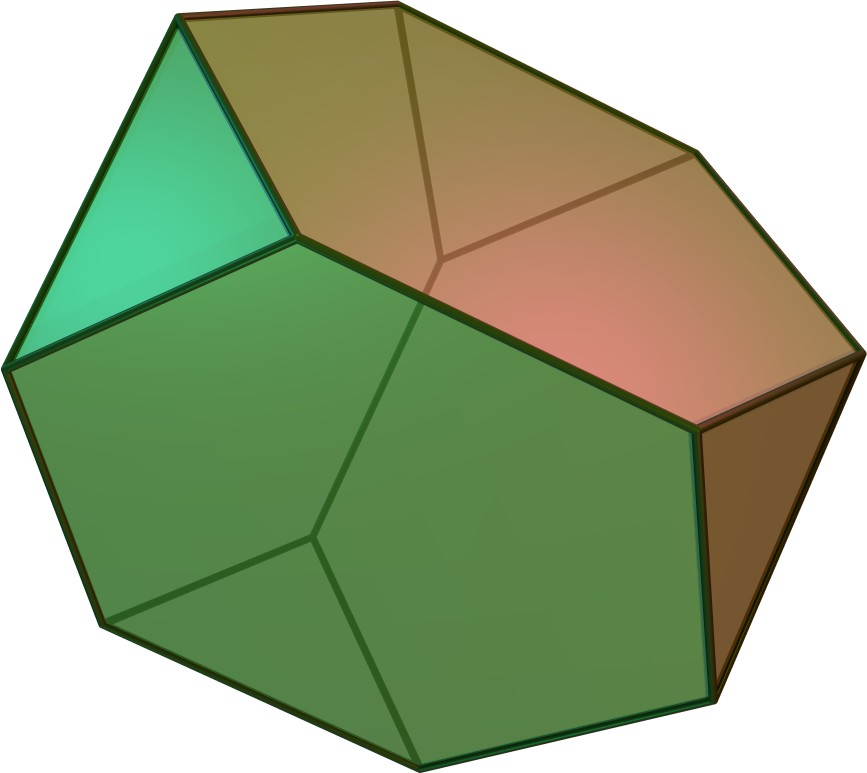
\includegraphics[width=1.5in]{TruncatedTetrahedron}
}
\subcaptionbox{\label{fig:TruncatedIcosahedron}}[.3\textwidth]{
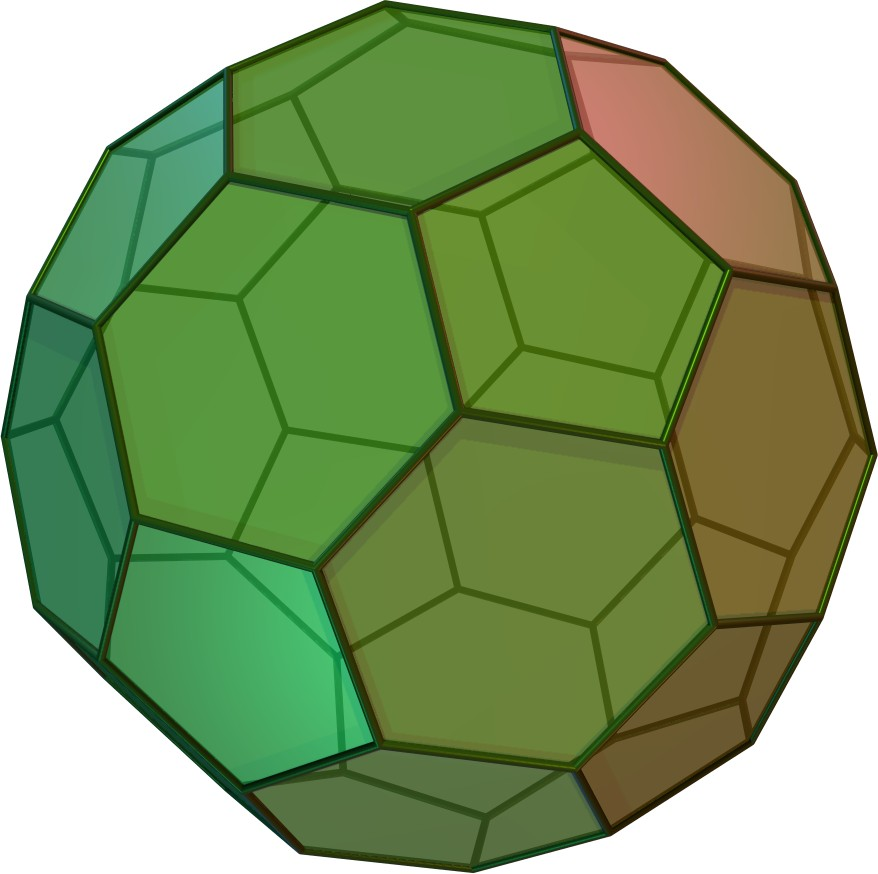
\includegraphics[width=1.5in]{TruncatedIcosahedron}}
\subcaptionbox{\label{fig:TruncatedDodecahedron}}[.3\textwidth]{
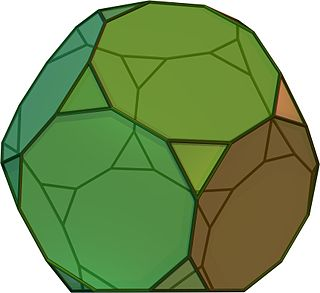
\includegraphics[width=1.5in]{TruncatedDodecahedron}}
\caption{Truncated tetrahedron, truncated icosahedron, and truncated dodecahedron. [Image source: \href{https://en.wikipedia.org/wiki/Truncated_tetrahedron}{Wikipedia}]}
\end{center}
\end{figure}

\end{section}